\documentclass[10pt,twocolumn]{article}

\usepackage[letterpaper,top=0.62in,bottom=0.68in,left=0.64in,right=0.64in,columnsep=0.28in]{geometry}
\usepackage[T1]{fontenc}
\usepackage{lmodern}
\usepackage{microtype}
\usepackage{amsmath,amssymb}
\usepackage{booktabs}
\usepackage{enumitem}
\usepackage{graphicx}
\usepackage{tabularx}
\usepackage{tikz}
\usepackage{xcolor}
\usepackage{url}
\usepackage[hidelinks]{hyperref}

\definecolor{paperblue}{HTML}{173A5E}
\definecolor{paperorange}{HTML}{C97B22}
\definecolor{papergreen}{HTML}{2F8F83}
\definecolor{papergray}{HTML}{6C7A89}

\hypersetup{
  pdftitle={CommCanary 0.4v: Fail Closed Evidence for Decision Fidelity Evaluation of Collective Trace Replay.},
  pdfauthor={Anshuman Agrawal},
  pdfsubject={Systems research on independently verifiable collective trace replay experiments},
  pdfkeywords={collective communication, trace replay, decision fidelity, reproducibility, NCCL},
  colorlinks=true,
  linkcolor=paperblue,
  citecolor=paperblue,
  urlcolor=paperblue
}

\setlength{\parindent}{1em}
\setlength{\parskip}{0pt}
\setlist{nosep,leftmargin=*}
\renewcommand{\arraystretch}{1.04}
\newcommand{\wname}[1]{\texttt{W-#1}}
\newcommand{\us}{\,\mu\mathrm{s}}

\title{\vspace{-1.5em}\bfseries\color{paperblue}
  CommCanary 0.4v: Fail Closed Evidence for Decision Fidelity\\
  Evaluation of Collective Trace Replay.}
\author{Anshuman Agrawal\\[-0.1em]
  \small CommCanary Project\\[-0.1em]
  \small\href{https://doi.org/10.5281/zenodo.21939041}{doi:10.5281/zenodo.21939041}}
\date{}

\begin{document}
\maketitle
\vspace{-1.7em}

\begin{abstract}
Collective communication traces can replace expensive distributed workloads in
controlled experiments, but replaying the right calls does not guarantee the
same configuration choice. CommCanary provides a fail-closed workflow for
freezing, selecting, archiving, and independently checking collective-trace
replay evidence. Its publication path binds a campaign to immutable attempts,
an explicit selection, a completeness verdict, a hash-identified archive, and
deterministic analysis. Missing or unstable evidence withholds the claim.

We compare four replay representations with a full workload on one node with
four NVIDIA A100 GPUs and eight NCCL configurations. The trusted join contains
all 280 selected cells. Communication-only replay does not preserve the
measured workload decision. \wname{canary} reaches 57.1\% pair agreement, below
the 64.3\% of \wname{micro}. Adding compute and communication concurrency
changes the ranking. \wname{shared-overlap} reaches 71.4\% agreement and
$\tau_b=0.708$, but still disagrees on 8 of 28 pairs.

A separate exact-work gate reports 26 of 28 agreeing pairs, or 92.86\%, with
$\tau_b=0.857$, one false negative, one false positive, 1.55\% median absolute
relative error, and 4.05\% p95 error. The persisted verdict is
\emph{inconclusive}, not pass. Bootstrap intervals cross frozen decision
boundaries, and one configuration exceeds the relative-IQR stability limit.
The evidence supports a measured negative result about communication-only
replay and an independently verifiable publication workflow. It does not
qualify CommCanary as a production gate, prove general decision preservation,
or establish savings from a reduced physical canary.
\end{abstract}

\section{Introduction}

Distributed machine learning and high-performance computing systems often
require a choice among collective algorithms, protocols, or library versions.
That choice depends on more than message size. Process arrival times, network
topology, endpoint resource use, operation order, and overlap with computation
can all change the ranking. MPI implementations therefore select among
multiple collective algorithms, and NCCL exposes algorithm and protocol
choices whose performance depends on workload context~\cite{mpi,nccl,thakur,vadhiyar}.
An isolated microbenchmark can measure a collective precisely while omitting
the execution conditions that determine the application choice.

Execution traces provide another way to study a workload. A trace can record
operations and dependencies; a simulator or replay engine can then execute the
recorded structure without rerunning the original application
\cite{chakra,mystique,astrasim,astrasim2,scalatrace,loggopsim}. The relevant
fidelity target still has to be stated. A tuning workflow usually asks which
configuration should be selected. Small timing error is not enough if replay
reverses two close configurations. High point agreement is also insufficient
when the measurements are unstable or uncertainty spans the decision boundary.

This work asks whether collective-trace replay preserves the pairwise
configuration decisions of a full workload, and whether the evidence path
refuses a positive claim when completeness, uncertainty, or stability is
inadequate.

CommCanary handles the evidence question first. A campaign is frozen before
execution. Each expected cell writes immutable attempts. A separate selection
identifies one terminal attempt for each cell. A completeness verdict checks
that the selected matrix is present, unambiguous, and successful. Raw evidence
is archived and hashed. Publication files are generated deterministically from
that selection. A failed boundary stops the claim path.

We use this workflow in two experiments. The first joins three complete
campaigns into 280 selected cells covering eight NCCL configurations and seven
workload profiles. It compares four replay representations with the full
workload. Communication-only \wname{canary} agrees on 16 of 28 configuration
pairs, or 57.1\%. Isolated \wname{micro} agrees on 18, or 64.3\%. A shared trace
replay with concurrent compute reaches 20, or 71.4\%. Concurrency changes the
measured ranking, but no proxy preserves all decisions.

The second experiment reconstructs the source-derived work exactly and
evaluates it with a policy frozen before analysis. Exact work reaches 26 of 28
pair agreement with low relative timing error. Every point criterion passes.
The gate still returns inconclusive because pair intervals cross tie boundaries
and the \texttt{nccl-2.20.5-tree-ll} configuration is unstable in three
representations. A favorable estimate is recorded without being promoted to a
supported qualification claim.

The paper contributes four items:

\begin{enumerate}
  \item a fail-closed evidence model for physical collective-replay experiments,
    with immutable attempts, explicit selection, completeness, archive binding,
    and deterministic publication;
  \item a complete 280-cell comparison showing that faithful communication-only
    replay is insufficient for the measured decision and that compute and
    communication concurrency changes the ranking;
  \item a predeclared exact-work gate that reports strong point estimates and the
    final inconclusive verdict; and
  \item an explicit separation between publication evidence, diagnostic
    evidence, incomplete integration records, and work that has not run.
\end{enumerate}

All physical observations come from a single node with four A100 GPUs. The
results do not establish multi-node behavior, expert-parallel replay,
congestion fidelity, CUDA-graph fidelity, vendor qualification, production-CI
readiness, or runtime savings from a reduced canary.

\section{Background and problem definition}

\subsection{Collective configuration depends on context}

Collective operations define group communication semantics while leaving
implementation strategy open~\cite{mpi}. Classic MPI work shows that no single
algorithm dominates across message sizes, process counts, and systems
\cite{thakur,vadhiyar}. NCCL provides topology-aware GPU collectives and allows
algorithm and protocol selection~\cite{nccl}. Our configuration set contains
two NCCL versions at default selection and six choices formed by crossing Ring
or Tree with LL, LL128, or Simple on NCCL 2.20.5.

An isolated microbenchmark is useful for transport characterization and
regression isolation. It intentionally removes application context. Concurrent
compute and communication can contend for endpoint resources and change the
critical path~\cite{overlap}. Arrival skew, explicit waits, dependencies, and
buffer lifetimes can also change which configuration is preferred. The
microbenchmark ranking is therefore an experimental result, not a default
model of the full-workload ranking.

\subsection{Trace replay and surrogate workloads}

Trace systems support different goals. ScalaTrace compresses and replays
communication traces~\cite{scalatrace}. LogGOPSim combines traces with an
analytical communication model~\cite{loggopsim}. ASTRA-SIM explores distributed
training systems through workload and network models~\cite{astrasim,astrasim2}.
Chakra defines an execution-trace schema for operations and dependencies,
while Mystique derives portable AI benchmarks from execution traces
\cite{chakra,mystique}. PARAM supplies communication benchmark and replay
tooling used by the experiment path~\cite{param}.

Trace portability does not decide the claim target. CommCanary tests decision
fidelity: whether a replay supports the same configuration choice as the source
workload under a frozen policy. The contribution is not a new trace format or
simulator. It is a decision-level evaluation coupled to a physical evidence
boundary that can withhold the claim.

\subsection{Decision fidelity}

Let $C$ be the measured configurations and $R$ a representation such as the
full workload, a microbenchmark, or a replay. For each unordered pair $(a,b)$,
a policy maps timing distributions to
\begin{equation}
  d_R(a,b) \in \{a \prec b,\; a \sim b,\; b \prec a\},
\end{equation}
where $\prec$ means faster and $\sim$ means an operational tie. Agreement
between representation $R$ and the full workload $F$ is
\begin{equation}
  A(R,F)=\binom{|C|}{2}^{-1}\sum_{a<b}
  \mathbf{1}[d_R(a,b)=d_F(a,b)].
\end{equation}

Eight configurations produce 28 pair decisions. We also report Kendall's
tie-adjusted statistic~\cite{kendall}:
\begin{equation}
  \tau_b=\frac{N_c-N_d}
  {\sqrt{(N_c+N_d+T_R)(N_c+N_d+T_F)}}.
\end{equation}
Here $N_c$ and $N_d$ count concordant and discordant pairs, while $T_R$ and
$T_F$ count pairs tied on only one side. Exact agreement requires the same
three-way label. Kendall $\tau_b$ discounts some tie disagreements. Reporting
both exposes cases where a representation preserves the non-tied order but
changes many decisions into ties.

The trusted join uses its analyzer's frozen IQR rule. A pair is tied when its
median difference is smaller than either configuration's IQR. The exact-work
gate is a separate experiment with a pair-specific tie band, bootstrap
intervals, and a stability requirement. Its thresholds are not applied
retroactively to the trusted join.

\subsection{Point estimates and verdicts}

Performance samples can be autocorrelated, multimodal, or sensitive to machine
state. Scientific benchmarking practice calls for a complete method, repeated
observations, and explicit uncertainty~\cite{benchmarking}. The exact-work gate
uses percentile-bootstrap intervals~\cite{efron} and a relative-IQR stability
limit. A point estimate can pass while its interval overlaps a tie or reversal
region. The policy then returns insufficient evidence instead of pass.

\section{CommCanary evidence model}

\subsection{Fail-closed publication path}

Figure~\ref{fig:path} shows the publication path. The boundaries remain
separate because each answers a different question.

\begin{enumerate}
  \item The campaign manifest freezes the matrix, environment identities,
    producer identities, policies, and expected cells before measurement.
  \item Each cell owns an immutable sequence of attempts. A retry appends a new
    attempt.
  \item A selection names the terminal attempt used for every expected cell
    and is itself hashed.
  \item A completeness verdict checks cardinality, identity, terminal status,
    and declared artifacts.
  \item An archive descriptor binds the retained raw evidence to exact bytes.
  \item The analyzer emits aggregate JSON and CSV, a paper fragment, and policy
    verdicts from the selected evidence.
\end{enumerate}

The absence of a completeness verdict is not an empty valid sample. A parser's
ability to compute a number does not authorize publication. Synthetic fixtures
test software behavior but do not enter physical claims. Operational notes may
explain an attempt, but cannot replace an aggregate or persisted verdict.

\begin{figure*}[t]
  \centering
  \resizebox{0.96\textwidth}{!}{
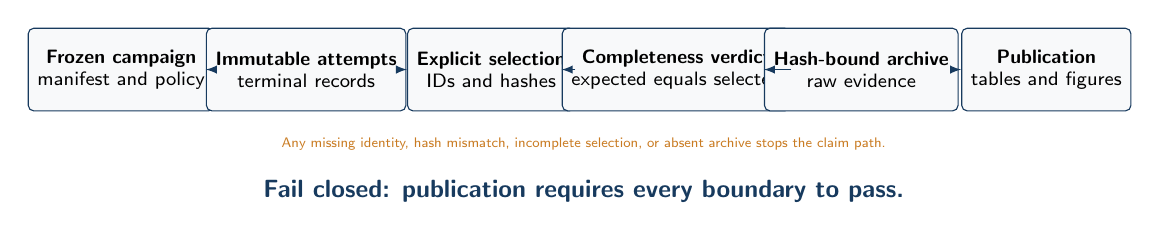
\begin{tikzpicture}[
  x=1cm,y=1cm,>=latex,
  box/.style={draw=paperblue,rounded corners=2pt,minimum width=2.05cm,
    minimum height=1.05cm,align=center,fill=paperblue!3,font=\sffamily\scriptsize},
  label/.style={font=\sffamily\tiny,text=papergray,align=center}
]
\node[box] (a) at (0,0) {\textbf{Frozen campaign}\\manifest and policy};
\node[box] (b) at (2.35,0) {\textbf{Immutable attempts}\\terminal records};
\node[box] (c) at (4.70,0) {\textbf{Explicit selection}\\IDs and hashes};
\node[box] (d) at (7.05,0) {\textbf{Completeness verdict}\\expected equals selected};
\node[box] (e) at (9.40,0) {\textbf{Hash-bound archive}\\raw evidence};
\node[box] (f) at (11.75,0) {\textbf{Publication}\\tables and figures};
\foreach \x/\y in {a/b,b/c,c/d,d/e,e/f} {\draw[->,paperblue] (\x) -- (\y);}
\node[label,text=paperorange] at (5.875,-0.95)
  {Any missing identity, hash mismatch, incomplete selection, or absent archive stops the claim path.};
\node[font=\sffamily\small\bfseries,text=paperblue] at (5.875,-1.55)
  {Fail closed: publication requires every boundary to pass.};
\end{tikzpicture}
}
  \caption{CommCanary publication path. Campaign identity, immutable attempts,
  selection, completeness, archive binding, and publication are separate
  gates. Missing or inconsistent evidence stops the claim path.}
  \label{fig:path}
\end{figure*}

\subsection{Evidence grades}

Table~\ref{tab:grades} separates the material used in this paper. Publication
evidence has a complete hash-bound campaign and generated analysis. Diagnostic
evidence supports a narrow observation without issuing a qualification verdict.
Failed integrations remain engineering records and are excluded from
quantitative results. Product studies that have not run are future work.

\begin{table*}[t]
\caption{Claim boundary by evidence grade.}
\label{tab:grades}
\centering\small
\begin{tabularx}{\textwidth}{@{}p{0.18\textwidth}p{0.40\textwidth}X@{}}
\toprule
Grade & Included material & Permitted interpretation \\
\midrule
Publication evidence & 280-cell trusted join and 8-cell exact-work gate &
Supports the measured comparison and gate observations only. \\
Diagnostic & Same-node source and replay timing with deterministic checks &
Supports reconstruction debugging; no qualification verdict or general claim. \\
Failed or incomplete integration & Attempts without a complete hash-bound
publication package & Excluded from quantitative results. An operational
failure is not scientific evidence. \\
Future work & Real vLLM or SGLang corpus, held-out physical canary, additional
nodes and congestion studies & Not evaluated and not implied by the present
artifacts. \\
\bottomrule
\end{tabularx}
\end{table*}

\subsection{Independent regeneration}

The evidence commit retains primary and reproduction directories for the
exact-work gate. Their \texttt{aggregate.csv}, \texttt{aggregate.json},
\texttt{decision-fidelity-verdict.json}, and \texttt{paper-fragment.md} files
have identical Git blob identities. This confirms that the checked-in
deterministic publication path produced the same bytes for the retained
inputs. It does not show that physical measurements reproduce on another
machine, and it does not turn a focused analyzer check into release readiness.

\section{Experimental methodology}

\subsection{Campaign inventory and hardware scope}

Table~\ref{tab:campaigns} lists the evidence packages. The main comparison
joins three campaigns from one four-GPU A100 node. Eight configurations, seven
workload profiles, and five selected repetitions produce 280 cells. Each cell
contributes 100 retained samples after warmup. The exact-work gate has one cell
per configuration and 20 measured iterations for every representation after
five warmups. The diagnostic contains one configuration and compares source
and replay on the same node.

All claims are conditioned on the measured node, workload, configuration set,
and campaign identity. No result is extrapolated to NVSwitch, another
accelerator generation, a multi-node fabric, or concurrent cluster traffic.

\begin{table*}[t]
\caption{Campaign inventory. Complete means that the manifest-bound
completeness verdict passed.}
\label{tab:campaigns}
\centering\scriptsize
\begin{tabularx}{\textwidth}{@{}p{0.18\textwidth}p{0.16\textwidth}p{0.34\textwidth}p{0.13\textwidth}X@{}}
\toprule
Package & Hardware scope & Matrix and sampling & Selection & Claim status \\
\midrule
Trusted comparison join & One node; 4 A100 GPUs & 8 configurations, 7
profiles, 5 selected repetitions per cell, 100 retained samples per cell &
280 of 280 cells & Complete comparative evidence \\
Exact-work gate & One node; 4 A100 GPUs & 8 configurations, 28 unordered
pairs, 20 measured iterations after 5 warmups & 8 of 8 cells & Point criteria
pass; final verdict inconclusive \\
Exact-work diagnostic & Same node; four ranks & 1 configuration, 20 source and
replay samples, 32 deterministic checks & 1 of 1 cell & Complete diagnostic;
no qualification verdict \\
\bottomrule
\end{tabularx}
\end{table*}

\subsection{Configurations}

The finite decision set contains NCCL 2.19.3 with default algorithm and
protocol selection, NCCL 2.20.5 with default selection, and NCCL 2.20.5 with
Ring or Tree crossed with LL, LL128, or Simple. The campaign identity freezes
versions and environment. These configurations are the eight choices evaluated
here, not a representative sample of all NCCL behavior.

\subsection{Representations}

The trusted join contains seven workload profiles. Four are compared directly
with the full workload.

\paragraph{\wname{micro}.} An isolated collective microbenchmark. It removes
workload computation and timing context.

\paragraph{\wname{canary}.} A faithful communication-only replay of recorded
collective requests and explicit waits. It preserves communication structure
but omits concurrent source computation.

\paragraph{\wname{canary-overlap}.} A configuration-specific overlap replay
that places compute around communication according to the captured schedule.

\paragraph{\wname{shared-overlap}.} An overlap replay driven by one shared
trace. Replayed work remains fixed while the NCCL configuration changes.

The full workload, \wname{full}, is the reference. The distinction between the
overlap representations matters because a configuration-specific trace can
encode configuration-dependent timing. A shared trace controls that source of
variation. Neither replay is presented as a reduced physical canary, and the
measured campaigns establish no runtime or artifact-size advantage over the
full workload.

\subsection{Trusted-join analysis}

Before aggregation, the analyzer validates result schemas, selected attempts,
campaign identities, and completeness. It computes retained timing
distributions for each workload and configuration cell. Configuration order
follows generated medians. Pair labels use the frozen IQR tie rule from
Section~2.3. We report the 28 exact pair labels and $\tau_b$. Quantitative
tables from the historical paper draft are excluded because their original
complete evidence was not retained.

\subsection{Exact-work decision gate}

The exact-work experiment evaluates source-derived execution, verified exact
work materialization, and control representations. Its policy was frozen
before evaluation. The domain is a single-node, four-A100 program with one
inflight all-reduce at a time, explicit waits, and source-observed contiguous
GEMM work.

Every representation has five warmups and 20 measured iterations. The policy
uses an independent 95\% percentile bootstrap with 2,000 resamples and seed
7411. A configuration is unstable when relative IQR exceeds 20\%. For source
medians $m_a$ and $m_b$, the pair tie band is
\begin{equation}
  \delta(a,b)=\max(10\us,\;0.05\min(m_a,m_b)).
\end{equation}

Point criteria require at least 80\% pair agreement, $\tau_b$ of at least 0.7,
no more than one false negative and one false positive, median and p95 absolute
relative errors below 10\% and 15\%, and at least two additional agreeing pairs
over each control. Passing these point criteria is necessary but not
sufficient. A pass can be withheld when bootstrap intervals cross decision
regions or when the stability condition fails.

\section{Results}

\subsection{Communication-only replay does not preserve the decision}

Table~\ref{tab:agreement} and Figures~\ref{fig:agreement} and
\ref{fig:kendall} report the trusted join. \wname{canary} agrees with
\wname{full} on 16 of 28 pairs, or 57.1\%, with $\tau_b=0.204$.
\wname{micro} agrees on 18 pairs, or 64.3\%, with $\tau_b=0.490$. Replaying
the request and wait structure without computation is therefore insufficient
for this measured decision. Under exact labels it performs worse than the
isolated microbenchmark.

The disagreement concerns configuration selection, not only absolute latency.
\wname{canary} places the full workload's worst measured configuration near the
front of its ranking. A replay can match call count and byte count while
changing the interference and synchronization that produce the ordering.

\begin{table}[t]
\caption{Agreement with \wname{full} over eight configurations.}
\label{tab:agreement}
\centering\small
\begin{tabular}{@{}lrr@{}}
\toprule
Representation & Pair agreement & Kendall $\tau_b$ \\
\midrule
\wname{micro} & 18/28 (64.3\%) & 0.490 \\
\wname{canary} & 16/28 (57.1\%) & 0.204 \\
\wname{canary-overlap} & 15/28 (53.6\%) & 0.677 \\
\wname{shared-overlap} & 20/28 (71.4\%) & 0.708 \\
\bottomrule
\end{tabular}
\end{table}

\begin{figure}[t]
  \centering
  \resizebox{0.98\columnwidth}{!}{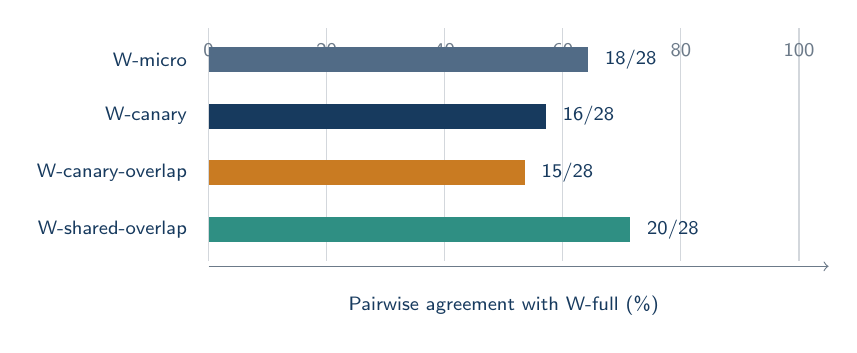
\begin{tikzpicture}[x=0.075cm,y=0.72cm,font=\sffamily\scriptsize]
\draw[->,papergray] (0,-0.65) -- (105.0,-0.65);
\draw[papergray!30] (0.0,-0.55) -- (0.0,3.55) node[below=2pt,text=papergray] {0};
\draw[papergray!30] (20.0,-0.55) -- (20.0,3.55) node[below=2pt,text=papergray] {20};
\draw[papergray!30] (40.0,-0.55) -- (40.0,3.55) node[below=2pt,text=papergray] {40};
\draw[papergray!30] (60.0,-0.55) -- (60.0,3.55) node[below=2pt,text=papergray] {60};
\draw[papergray!30] (80.0,-0.55) -- (80.0,3.55) node[below=2pt,text=papergray] {80};
\draw[papergray!30] (100.0,-0.55) -- (100.0,3.55) node[below=2pt,text=papergray] {100};
\node[anchor=east,text=paperblue] at (-2.000,3) {W-micro};
\fill[paperblue!75] (0,2.78) rectangle (64.285714,3.22);
\node[anchor=west,text=paperblue] at (65.485714,3) {18/28};
\node[anchor=east,text=paperblue] at (-2.000,2) {W-canary};
\fill[paperblue] (0,1.78) rectangle (57.142857,2.22);
\node[anchor=west,text=paperblue] at (58.342857,2) {16/28};
\node[anchor=east,text=paperblue] at (-2.000,1) {W-canary-overlap};
\fill[paperorange] (0,0.78) rectangle (53.571429,1.22);
\node[anchor=west,text=paperblue] at (54.771429,1) {15/28};
\node[anchor=east,text=paperblue] at (-2.000,0) {W-shared-overlap};
\fill[papergreen] (0,-0.22) rectangle (71.428571,0.22);
\node[anchor=west,text=paperblue] at (72.628571,0) {20/28};
\node[text=paperblue] at (50.000,-1.35) {Pairwise agreement with W-full (\%)};
\end{tikzpicture}
}
  \caption{Exact three-way pair agreement with the full-workload decision. No
  measured proxy reaches 80\%.}
  \label{fig:agreement}
\end{figure}

\begin{figure}[t]
  \centering
  \resizebox{0.98\columnwidth}{!}{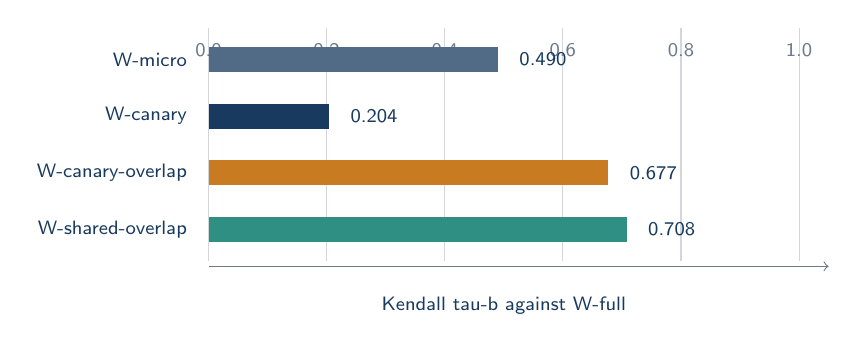
\begin{tikzpicture}[x=7.500cm,y=0.72cm,font=\sffamily\scriptsize]
\draw[->,papergray] (0,-0.65) -- (1.05,-0.65);
\draw[papergray!30] (0.0,-0.55) -- (0.0,3.55) node[below=2pt,text=papergray] {0.0};
\draw[papergray!30] (0.2,-0.55) -- (0.2,3.55) node[below=2pt,text=papergray] {0.2};
\draw[papergray!30] (0.4,-0.55) -- (0.4,3.55) node[below=2pt,text=papergray] {0.4};
\draw[papergray!30] (0.6,-0.55) -- (0.6,3.55) node[below=2pt,text=papergray] {0.6};
\draw[papergray!30] (0.8,-0.55) -- (0.8,3.55) node[below=2pt,text=papergray] {0.8};
\draw[papergray!30] (1.0,-0.55) -- (1.0,3.55) node[below=2pt,text=papergray] {1.0};
\node[anchor=east,text=paperblue] at (-0.020,3) {W-micro};
\fill[paperblue!75] (0,2.78) rectangle (0.490000,3.22);
\node[anchor=west,text=paperblue] at (0.510000,3) {0.490};
\node[anchor=east,text=paperblue] at (-0.020,2) {W-canary};
\fill[paperblue] (0,1.78) rectangle (0.204000,2.22);
\node[anchor=west,text=paperblue] at (0.224000,2) {0.204};
\node[anchor=east,text=paperblue] at (-0.020,1) {W-canary-overlap};
\fill[paperorange] (0,0.78) rectangle (0.677000,1.22);
\node[anchor=west,text=paperblue] at (0.697000,1) {0.677};
\node[anchor=east,text=paperblue] at (-0.020,0) {W-shared-overlap};
\fill[papergreen] (0,-0.22) rectangle (0.708000,0.22);
\node[anchor=west,text=paperblue] at (0.728000,0) {0.708};
\node[text=paperblue] at (0.500,-1.35) {Kendall tau-b against W-full};
\end{tikzpicture}
}
  \caption{Tie-adjusted Kendall correlation with the full-workload ordering.
  Correlation and exact three-way agreement answer different questions.}
  \label{fig:kendall}
\end{figure}

\subsection{Concurrency changes the ranking}

Adding overlap changes both pair agreement and tie structure.
\wname{canary-overlap} agrees on 15 of 28 pairs, or 53.6\%, while its
$\tau_b$ is 0.677. The low exact agreement and higher rank correlation are
consistent with many pairs becoming policy ties. The remaining non-tied order
is more concordant even though the exact labels differ.

\wname{shared-overlap} is the strongest measured proxy at 20 of 28 agreement,
or 71.4\%, with $\tau_b=0.708$. It gains two agreeing pairs over
\wname{micro} and four over \wname{canary}. Holding concurrent work constant
while changing the NCCL configuration materially changes the result. Eight pair
decisions still disagree with \wname{full}, so the experiment does not qualify
overlap replay.

The trusted join is descriptive and predates the separate exact-work policy.
We do not apply a new threshold after observing the result. The complete
ordering instead motivates the predeclared gate.

\subsection{Exact work has strong point estimates}

Exact work agrees on 26 of 28 pairs, or 92.86\%, with $\tau_b=0.857$. It
records one false negative and one false positive. Median absolute relative
error is 1.55\%, and p95 error is 4.05\%. It gains seven agreeing pairs over
the isolated control and sixteen over the stratified control. Every point
criterion passes, as Table~\ref{tab:criteria} records.

These estimates show that exact-work reconstruction is substantially closer to
the source ordering than the controls in this campaign. They do not determine
the final claim because a pair decision also requires a supported interval and
stable input measurements.

\begin{table*}[t]
\caption{Predeclared exact-work point criteria. Every point row passes, but the
final verdict also requires supported uncertainty and stability.}
\label{tab:criteria}
\centering\small
\begin{tabular}{@{}lrrc@{}}
\toprule
Criterion & Observed & Required & Point status \\
\midrule
Pair agreement & 92.86\% & at least 80\% & pass \\
Kendall $\tau_b$ & 0.857 & at least 0.7 & pass \\
False negatives & 1 & at most 1 & pass \\
False positives & 1 & at most 1 & pass \\
Median absolute relative error & 1.55\% & at most 10\% & pass \\
p95 absolute relative error & 4.05\% & at most 15\% & pass \\
Agreement advantage over isolated & 7 pairs & at least 2 pairs & pass \\
Agreement advantage over stratified & 16 pairs & at least 2 pairs & pass \\
\bottomrule
\end{tabular}
\end{table*}

\subsection{The predeclared verdict is inconclusive}

The persisted outcome is \emph{inconclusive}. Two conditions prevent pass.

First, bootstrap intervals for several exact-work pair differences cross the
frozen decision regions. Figure~\ref{fig:inconclusive} normalizes representative
differences and 95\% intervals by each pair's tie threshold. An interval below
$-1$ supports the second configuration, an interval above $+1$ supports the
first, and an interval contained within $[-1,+1]$ supports a tie. Crossing
those regions leaves the label unsupported.

Second, \texttt{nccl-2.20.5-tree-ll} exceeds the 20\% relative-IQR limit in
source at 47.5\%, exact work at 32.3\%, and the stratified control at 50.4\%.
The instability appears in more than the candidate representation. The
campaign cannot support a clean qualification involving that configuration
under the frozen policy.

The supported reading is asymmetric. Exact work is promising and closer to the
source decisions than the controls in this campaign. The evidence does not
show that the gate passed, that decision preservation is proven, or that exact
work is a qualified production oracle.

\begin{figure*}[t]
  \centering
  \resizebox{0.95\textwidth}{!}{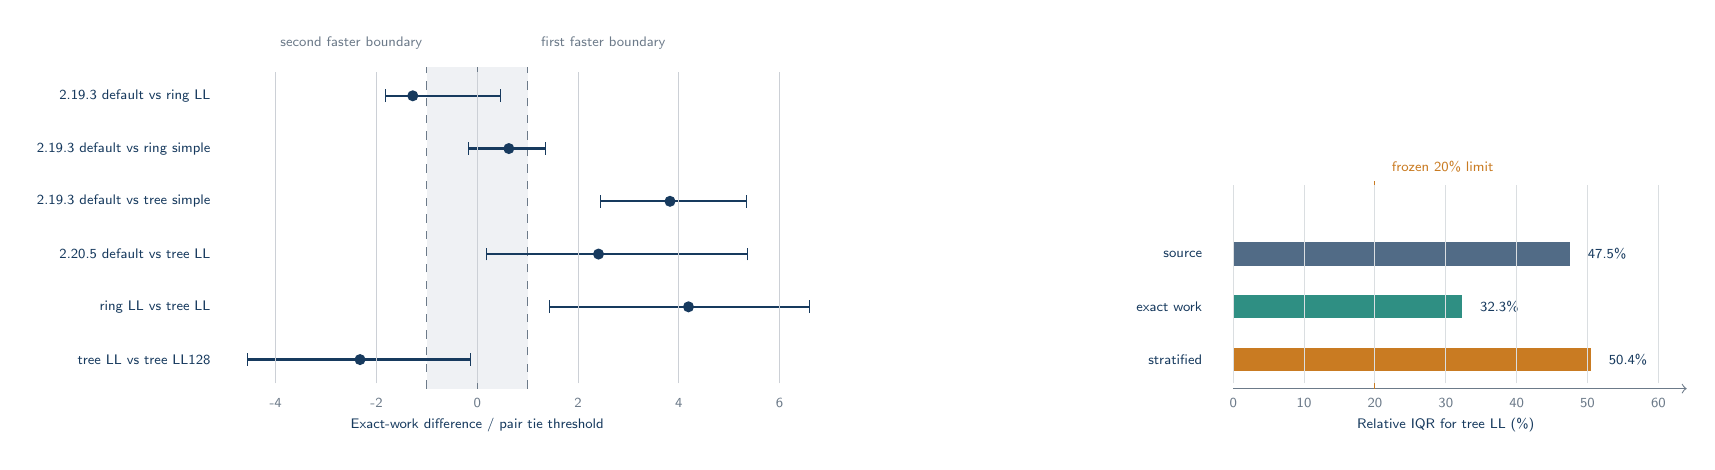
\begin{tikzpicture}[x=0.64cm,y=0.67cm,font=\sffamily\tiny]
\begin{scope}[xshift=0cm]
\fill[paperblue!7] (-1,-0.55) rectangle (1,5.55);
\draw[dashed,papergray] (-1,-0.55) -- (-1,5.55);
\draw[dashed,papergray] (1,-0.55) -- (1,5.55);
\draw[papergray] (0,-0.55) -- (0,5.55);
\node[text=papergray] at (-2.5,6.0) {second faster boundary};
\node[text=papergray] at (2.5,6.0) {first faster boundary};
\node[anchor=east,text=paperblue] at (-5.1,5) {2.19.3 default vs ring LL};
\draw[paperblue,thick] (-1.823755,5) -- (0.467433,5);
\draw[paperblue] (-1.823755,4.88) -- (-1.823755,5.12);
\draw[paperblue] (0.467433,4.88) -- (0.467433,5.12);
\fill[paperblue] (-1.279693,5) circle (2pt);
\node[anchor=east,text=paperblue] at (-5.1,4) {2.19.3 default vs ring simple};
\draw[paperblue,thick] (-0.172848,4) -- (1.353979,4);
\draw[paperblue] (-0.172848,3.88) -- (-0.172848,4.12);
\draw[paperblue] (1.353979,3.88) -- (1.353979,4.12);
\fill[paperblue] (0.626575,4) circle (2pt);
\node[anchor=east,text=paperblue] at (-5.1,3) {2.19.3 default vs tree simple};
\draw[paperblue,thick] (2.448686,3) -- (5.336694,3);
\draw[paperblue] (2.448686,2.88) -- (2.448686,3.12);
\draw[paperblue] (5.336694,2.88) -- (5.336694,3.12);
\fill[paperblue] (3.824271,3) circle (2pt);
\node[anchor=east,text=paperblue] at (-5.1,2) {2.20.5 default vs tree LL};
\draw[paperblue,thick] (0.191625,2) -- (5.370121,2);
\draw[paperblue] (0.191625,1.88) -- (0.191625,2.12);
\draw[paperblue] (5.370121,1.88) -- (5.370121,2.12);
\fill[paperblue] (2.405962,2) circle (2pt);
\node[anchor=east,text=paperblue] at (-5.1,1) {ring LL vs tree LL};
\draw[paperblue,thick] (1.431992,1) -- (6.592720,1);
\draw[paperblue] (1.431992,0.88) -- (1.431992,1.12);
\draw[paperblue] (6.592720,0.88) -- (6.592720,1.12);
\fill[paperblue] (4.191571,1) circle (2pt);
\node[anchor=east,text=paperblue] at (-5.1,0) {tree LL vs tree LL128};
\draw[paperblue,thick] (-4.564887,0) -- (-0.134371,0);
\draw[paperblue] (-4.564887,-0.12) -- (-4.564887,0.12);
\draw[paperblue] (-0.134371,-0.12) -- (-0.134371,0.12);
\fill[paperblue] (-2.326733,0) circle (2pt);
\draw[papergray!35] (-4,-0.45) -- (-4,5.45);\node[below,text=papergray] at (-4,-0.55) {-4};
\draw[papergray!35] (-2,-0.45) -- (-2,5.45);\node[below,text=papergray] at (-2,-0.55) {-2};
\draw[papergray!35] (0,-0.45) -- (0,5.45);\node[below,text=papergray] at (0,-0.55) {0};
\draw[papergray!35] (2,-0.45) -- (2,5.45);\node[below,text=papergray] at (2,-0.55) {2};
\draw[papergray!35] (4,-0.45) -- (4,5.45);\node[below,text=papergray] at (4,-0.55) {4};
\draw[papergray!35] (6,-0.45) -- (6,5.45);\node[below,text=papergray] at (6,-0.55) {6};
\node[text=paperblue] at (0,-1.25) {Exact-work difference / pair tie threshold};
\end{scope}
\begin{scope}[xshift=9.6cm,x=0.09cm]
\draw[->,papergray] (0,-0.55) -- (64,-0.55);
\draw[dashed,paperorange] (20,-0.55) -- (20,3.45);
\node[text=paperorange,anchor=west] at (21,3.65) {frozen 20\% limit};
\node[anchor=east,text=paperblue] at (-3,2) {source};
\fill[paperblue!75] (0,1.78) rectangle (47.473101,2.22);
\node[anchor=west,text=paperblue] at (48.673101,2) {47.5\%};
\node[anchor=east,text=paperblue] at (-3,1) {exact work};
\fill[papergreen] (0,0.78) rectangle (32.277479,1.22);
\node[anchor=west,text=paperblue] at (33.477479,1) {32.3\%};
\node[anchor=east,text=paperblue] at (-3,0) {stratified};
\fill[paperorange] (0,-0.22) rectangle (50.428571,0.22);
\node[anchor=west,text=paperblue] at (51.628571,0) {50.4\%};
\draw[papergray!25] (0,-0.45) -- (0,3.3);\node[below,text=papergray] at (0,-0.55) {0};
\draw[papergray!25] (10,-0.45) -- (10,3.3);\node[below,text=papergray] at (10,-0.55) {10};
\draw[papergray!25] (20,-0.45) -- (20,3.3);\node[below,text=papergray] at (20,-0.55) {20};
\draw[papergray!25] (30,-0.45) -- (30,3.3);\node[below,text=papergray] at (30,-0.55) {30};
\draw[papergray!25] (40,-0.45) -- (40,3.3);\node[below,text=papergray] at (40,-0.55) {40};
\draw[papergray!25] (50,-0.45) -- (50,3.3);\node[below,text=papergray] at (50,-0.55) {50};
\draw[papergray!25] (60,-0.45) -- (60,3.3);\node[below,text=papergray] at (60,-0.55) {60};
\node[text=paperblue] at (30,-1.25) {Relative IQR for tree LL (\%)};
\end{scope}
\end{tikzpicture}
}
  \caption{Why the exact-work verdict is inconclusive. Representative 95\%
  intervals cross decision regions, and the tree-LL configuration violates the
  frozen stability limit.}
  \label{fig:inconclusive}
\end{figure*}

\subsection{Same-node diagnostic}

A separate one-cell diagnostic compares retained source and replay timing for
one exact-work capsule. The source median is $1{,}434.112\us$ and the replay
median is $1{,}541.0015\us$. The signed difference is $+106.8895\us$, or
$+7.4533578967\%$. All 32 deterministic checks pass across four ranks.
Table~\ref{tab:diagnostic} states the complete narrow claim.

The diagnostic confirms deterministic reconstruction checks and a same-node
timing comparison. It has no multi-configuration full-workload matrix. It
cannot issue a qualification verdict or substitute for the inconclusive
decision gate.

\begin{table}[t]
\caption{Exact-work diagnostic. No qualification verdict is issued.}
\label{tab:diagnostic}
\centering\small
\begin{tabularx}{\columnwidth}{@{}lX@{}}
\toprule
Item & Result \\
\midrule
Source median & $1{,}434.1120\us$ \\
Replay median & $1{,}541.0015\us$ \\
Signed difference & $+106.8895\us$ ($+7.4534\%$) \\
Source / replay IQR & $9.2160 / 8.9725\us$ \\
Deterministic checks & 32 passed across 4 ranks \\
Claim status & diagnostic; physical fidelity unproven; verdict not issued \\
\bottomrule
\end{tabularx}
\end{table}

\section{Interpretation}

\subsection{A trace encodes a causal hypothesis}

A communication trace selects the workload properties assumed to determine
the configuration choice. The communication-only representation assumes that
collective type, size, order, and synchronization are sufficient. The trusted
join rejects that assumption for the measured case. The operation stream can
be faithful at the communication interface while omitting concurrent work that
changes endpoint contention and critical-path timing.

The overlap results narrow the diagnosis. Adding concurrency does not improve
every metric. The configuration-specific overlap replay has fewer exact matches
than the microbenchmark because its tie structure changes. The shared-trace
variant performs best when concurrent work is held constant across
configurations. The overlap schedule, its dependence on configuration, and the
tie policy all affect the claim. Including overlap is necessary for this case
but is not a complete fidelity recipe.

\subsection{Decision fidelity differs from timing fidelity}

Absolute error and decision fidelity can diverge. Two configurations may differ
by less than measurement variability. A replay can have small percentage error
and reverse them, or a common timing bias and preserve their order. We report
pair labels, rank correlation, false-negative and false-positive counts, and
timing errors separately.

This distinction explains the exact-work outcome. Low median and p95 errors are
favorable, but the gate asks whether each operational decision is supported
under uncertainty. A 92.86\% point agreement is not a 92.86\% probability that
the replay is correct. An interval can invalidate the point label.

\subsection{Fail-closed evidence changes the default}

Experiment scripts often make it easy to produce a number. Missing runs can
disappear during aggregation, and retries can overwrite failures. A fail-closed
path makes incompleteness visible, preserves failed attempts, and requires
explicit selection before analysis. It adds operational work and metadata, but
it lets a later reader distinguish a complete negative result from an
incomplete favorable subset.

The exact-work verdict is the direct example. A threshold-only summary would
report that every numeric row passed. Because uncertainty and stability are
policy conditions, the retained conclusion is inconclusive.

\subsection{Unsupported conclusions}

The evidence does not show that a reduced physical canary is cheaper than the
full workload. Replay proxies are not a completed product corpus, and no
held-out physical regression study is present. The checked-in publication
package has no real vLLM or SGLang application campaign. Exact work is a
positive reconstruction control, not evidence that minimization succeeded.

Communication-only replay is not universally useless. The result shows
insufficiency for one measured single-node, four-A100 decision matrix. Such
replay can still help with debugging, transport isolation, or reproduction of a
call sequence when the claim remains at that level.

\section{Threats to validity and limitations}

\paragraph{Single system and workload.} All physical data comes from one
four-A100 PCIe node and one source-derived workload family. GPU topology, CPU
placement, software versions, thermal state, and site configuration may affect
the ranking. The result does not generalize to multi-node systems, NVSwitch,
other GPU generations, or vendor qualification.

\paragraph{Finite configuration set.} The decision object contains eight NCCL
configurations. It does not cover every environment variable, channel count,
topology override, message size, or collective library. Adding configurations
changes the number and difficulty of pair decisions.

\paragraph{Tie-policy sensitivity.} The trusted join uses an IQR rule. The
exact-work gate uses a pair-specific absolute or relative band with bootstrap
uncertainty. Both policies were frozen for their experiments, but another
operational tie definition could change labels. Exact counts and $\tau_b$ are
reported so the effect remains visible.

\paragraph{Measurement dependence.} Repeated timings within one process may be
dependent. The independent percentile bootstrap is a predeclared approximation,
not a universal model of system noise. A block or hierarchical bootstrap may
be preferable when temporal dependence is strong. Replication across nodes and
days remains future work.

\paragraph{Shared implementation.} A defect shared by source capture,
materialization, and verification could evade deterministic checks. Hash
binding proves byte identity, not semantic correctness. Independent producers,
differential implementations, and application invariants would provide
stronger controls.

\paragraph{Researcher choices.} Explicit selection and completeness reduce
post-hoc cell dropping, but campaign design, configuration choice, and policy
thresholds remain researcher decisions. The exact-work gate freezes thresholds
before analysis. The trusted join is a measured comparison, not a formal gate
defined after the result.

\paragraph{Publication boundary.} The paper uses generated artifacts retained
at a specific evidence commit. Older narrative measurements without complete
evidence are excluded. This avoids unsupported reuse, although it omits
historical observations that cannot now be independently reconstructed.

\section{Artifact availability and reproducibility}

The source repository is available at
\url{https://github.com/iemAnshuman/CommCanary}. The paper binds evidence
inspection to commit
\begin{center}
\texttt{c133ad3fb5883100cb8622b597d5b6233b5efca1}.
\end{center}
The version DOI is \href{https://doi.org/10.5281/zenodo.21939041}
{10.5281/zenodo.21939041}; the concept DOI is
\href{https://doi.org/10.5281/zenodo.21939040}{10.5281/zenodo.21939040}.

Campaigns retain their own manifest, selection, completeness, archive, and
repository identities. The outer evidence commit and source tree used to
prepare the paper are separate states. The trusted join is under
\path{experiments/rostam/results/publications/}. The exact-work diagnostic is
under \path{experiments/rostam/results/exact-work-artifacts/publication/}.
The authoritative directory names are:

\begin{itemize}
  \item \path{trusted-join-core-shared-overlap-primary/};
  \item \texttt{decision-gate-20260801-r3-}\allowbreak
    \texttt{analysis-1300d12-primary/};
  \item the corresponding reproduction directory; and
  \item \path{qualification-exact-20260730-r3-primary/}.
\end{itemize}

The supplied source-reconstruction scripts regenerate every vector figure from
\texttt{evidence/verified\_metrics.json}. That compact snapshot records verified
values and their paper binding. It does not replace immutable result
directories. Reproducing physical timings still requires recorded hardware and
software; deterministic analysis does not imply hardware-independent
measurements.

No commit, push, issue, Zenodo publication, DOI reservation, or release
metadata change is performed by the source tree. A focused analyzer or test run
must not be described as full release readiness.

\section{Related work}

\paragraph{Collective algorithms and tuning.} MPI defines collective semantics
but leaves the algorithm to the implementation~\cite{mpi}. MPICH studies show
why message size and process count affect algorithm selection~\cite{thakur}.
Performance models seek to predict or tune these choices~\cite{vadhiyar}. NCCL
provides GPU collectives and configurable algorithms and protocols~\cite{nccl};
NCCL Tests supplies operation-level measurements~\cite{nccltests}. CommCanary
uses the full-workload decision as the reference and tests whether a trace
representation preserves it.

\paragraph{Trace representation and replay.} ScalaTrace retains replay
capability while compressing communication traces~\cite{scalatrace}.
LogGOPSim simulates trace-driven communication at scale~\cite{loggopsim}.
ASTRA-SIM models distributed-learning workloads and networks
\cite{astrasim,astrasim2}. Chakra provides an execution-trace graph, Mystique
derives portable benchmarks from execution traces, and PARAM provides benchmark
and replay machinery~\cite{chakra,mystique,param}. CommCanary focuses on a
failure mode that these representations do not remove: a valid communication
trace can still change the configuration decision when it omits causal workload
context.

\paragraph{Compute and communication concurrency.} Earlier work measures the
resource interaction between computation and collective communication and
develops overlap mechanisms~\cite{overlap}. CommCanary does not introduce
another overlap engine. The experiments show that removing or changing overlap
alters which NCCL configuration appears preferable in the measured case.

\paragraph{Reduction and workload minimization.} Delta debugging removes input
while preserving a predicate~\cite{ddmin}. A future reduced canary can use a
similar objective: remove trace regions while preserving a decision-fidelity
predicate. The publication evidence contains no completed reduced physical
canary or cost result, so minimization remains a design direction.

\paragraph{Statistical comparison.} Benchmarking guidance warns against
selective statistics and incomplete variability reports~\cite{benchmarking}.
We pair exact decisions with Kendall's statistic~\cite{kendall} and use a
predeclared bootstrap procedure~\cite{efron}. Uncertainty and stability are
verdict conditions instead of annotations added after a point estimate.

\section{Conclusion}

The 280-cell comparison gives a clear negative result for communication-only
replay on the measured single-node, four-A100 system. \wname{canary} reaches
57.1\% pair agreement, below the isolated microbenchmark. Compute and
communication concurrency changes the ranking. The strongest shared-overlap
replay reaches 71.4\% but disagrees on eight pairs.

Exact work is much closer to the source ordering. Its 92.86\% agreement,
$\tau_b=0.857$, and low relative errors pass every point threshold. The final
outcome remains inconclusive because pair uncertainty crosses decision
boundaries and one configuration violates the stability limit.

The supported contribution is an independently verifiable, fail-closed
evidence workflow and a measured result about the role of concurrency.
Production qualification, reduced-canary savings, held-out regression safety,
application product studies, and generalization beyond the measured system
remain open.

\bibliographystyle{unsrt}
\bibliography{references}

\appendix
\section{Campaign identities}

Table~\ref{tab:identities} lists abbreviated campaign identities. Full SHA-256
values remain in \texttt{evidence/verified\_metrics.json} and authoritative
repository artifacts. M, S, C, and R denote manifest, selection, completeness
verdict, and repository commit.

\begin{table}[h]
\caption{Abbreviated manifest-bound campaign identities.}
\label{tab:identities}
\centering\scriptsize
\begin{tabularx}{\columnwidth}{@{}p{0.42\columnwidth}X@{}}
\toprule
Run / campaign & Bound identities \\
\midrule
core-20260724-r7 / rostam-core & M 3bd321ec960c; S d01db822c8e9; C 46d8012b3594; R 2855275288e6 \\
shared-replay-20260720-r2 / rostam-shared-replay & M a402a4ec73ea; S a1e876861f7f; C b6cd1aae4cfb; R 2855275288e6 \\
overlap-20260724-r1 / rostam-overlap & M 5d5eb9f4822e; S e012e40613f5; C 5b153d0452df; R 2855275288e6 \\
decision-gate-20260801-r3 / rostam-decision-gate & M 1b1909b3e856; S c675e42e34e4; C 6377a65bb057; R 4585318ac244 \\
qualification-exact-20260730-r3 / rostam-qualification-exact & M c0bc2e6a9ecb; S bf23480f39dd; C 593772c09020; R 9b1e58aef91e \\
\bottomrule
\end{tabularx}
\end{table}

\section{Trusted-join regeneration}

The generated publication fragment retains the analyzer invocation with its
exact argument order. The complete command is included in the source package
at \texttt{evidence/trusted\_join\_regeneration.txt}. It binds the core
campaign, primary selection and completeness verdict, joined evidence
directories, output directory, configuration identities, and median
thresholds.

\section{Claim ledger}

\paragraph{Supported comparative claim.} The trusted join contains 280 of 280
selected successful cells. Over the measured eight-configuration set,
\wname{shared-overlap} has the highest proxy agreement at 71.4\%.
Communication-only \wname{canary} reaches 57.1\%.

\paragraph{Supported gate observation.} Exact work has 26 of 28 point
agreement, $\tau_b=0.857$, one false negative, one false positive, 1.55\%
median absolute relative error, and 4.05\% p95 error. The persisted outcome is
inconclusive.

\paragraph{Supported diagnostic claim.} One same-node exact-work capsule has a
$1{,}434.112\us$ source median and a $1{,}541.0015\us$ replay median. All 32
deterministic checks pass. No qualification verdict is issued.

\paragraph{Not supported.} The paper does not support production
qualification, a passing decision gate, reduced-canary cost savings, held-out
safety, real vLLM or SGLang validation, multi-node or congestion fidelity,
CUDA-graph fidelity, general vendor qualification, or generalization beyond the
measured single-node, four-A100 scope.

\end{document}
